\chapter{Evaluaci\'on de nuestra propuesta}
\label{sec:evaluacion}


\begin{table}[!t]
\begin{small}
\begin{center}
\begin{tabular}{|l|r|r|r|r|r|}
\hline
\multirow{2}{*}{Referring Expressions} & \multicolumn{2}{|c|}{Corpus} & \multicolumn{2}{|c|}{Algorithm} & Accuracy \\ \cline{2-6} 
 & \#Cor & \multicolumn{1}{|c|}{\%Cor} & \multicolumn{1}{|c|}{\#Alg} & \multicolumn{1}{|c|}{\%Alg} & \multicolumn{1}{|c|}{\%Acc} \\
\hline
ball,green                                    & 91 & 65.00 & 6376 & 63.76 & 63.76 \\
ball,green,small                              & 23 & 16.43 & 3440 & 34.40 & 16.43 \\
ball,green,small,on-top(blue,cube,large)      &  8 &  5.71 &    0 &  0.00 &  0.00\\
ball,green,on-top(blue,cube)                  &  5 &  3.57 &    0 &  0.00 &  0.00\\
ball,green,on-top(blue,cube,large)            &  5 &  3.57 &    0 &  0.00 &  0.00\\
ball,green,small,on-top(blue,cube)            &  2 &  1.43 &    0 &  0.00 &  0.00\\
ball,on-top(cube)                             &  1 &  0.71 &   27 &  0.27 &  0.27 \\
ball,green,small,on-top(blue,cube,large,left) &  1 &  0.71 &    0 &  0.00 &  0.00\\
ball,small,on-top(cube,large)	              &  1 &  0.71 &    2 &  0.02 &  0.02 \\
ball,green,top                                &  1 &  0.71 &    0 &  0.00 &  0.00\\
ball,small,on-top(cube)                       &  1 &  0.71 &    3 &  0.03 &  0.03 \\
ball,green,on-top(cube)                       &  1 &  0.71 &    0 &  0.00 &  0.00\\
ball,front,green                              &  0 &  0.00 &   97 &  0.97 &  0.00\\
ball,front,green,small                        &  0 &  0.00 &   13 &  0.13 &  0.00\\
ball,front,top                                &  0 &  0.00 &   12 &  0.12 &  0.00\\
ball,green,left	                              &  0 &  0.00 &   11 &  0.11 &  0.00\\
ball,top                                      &  0 &  0.00 &   10 &  0.10 &  0.00\\
ball,green,left,small                         &  0 &  0.00 &    5 &  0.05 &  0.00\\
ball,left,top                                 &  0 &  0.00 &    2 &  0.02 &  0.00\\
ball,small,top                                &  0 &  0.00 &    1 &  0.01 &  0.00\\
ball,front,on-top(cube,left)                  &  0 &  0.00 &    1 &  0.01 &  0.00\\
\hline
Total & 140 & 100.00 & 10000 & 100 & 80.51 \\
\hline
\end{tabular}
\caption{REs in the corpus and those produced by our algorithm for Figure~\ref{GRE3D7-stimulus}\label{results-algo-fig3}}
\vspace*{-.5cm}
\end{center}
\end{small}
\end{table}

%We present a quantitative evaluation of the algorithm proposed. 
%In particular, we show that the probabilistic refinement algorithm with overspecification is able to generate a distribution of REs similar to that observed in corpora.
%, even when no corpus specific for a given target object is available. 
%We discuss in detail the experiments we run for the scene shown in Figure~\ref{GRE3D7-stimulus} (Scene 3 in the GRE3D7 corpus), then summarize the results for the other seven scenes we used for testing. 

Se presenta una evaluaci\'on cuantitativa del algoritmo propuesto.
En particular, se muestra que el algoritmo de refinamiento probabil\'{i}stico con especificaci\'on excesiva es capaz de generar una distribuci\'on similar a la observada en los corpus.
%, Incluso cuando no se dispone de corpus espec\'{i}fica para un objeto de destino determinado.
Se discute en detalle los experimentos ejecutados para la escena se muestra en la Figura~\ref{GRE3D7-stimulus}  (escena 3 en el corpus GRE3D7), a continuaci\'on, un resumen de los resultados de las otras siete escenas que utilizamos para las pruebas.



%Using \puse\ learned as described in Section~\ref{sec:learning} and running 
%our algorithm 10000 times, we obtain 14 different referring expressions 
%for Figure~\ref{GRE3D7-stimulus}.  It is already interesting to see that with the 
%\puse\ values learned from the corpus the algorithm generates only a small set of ER with a high probability. 
%Of these 14 different REs, 5 are the most frequent REs found in the corpus of 140 REs associated to the Scene; indeed, 98\% of the utterances generated by the algorithm for this scene appear in the corpus.  
%The remaining 9 REs generated by the algorithm, not present in the corpora, are very natural as can be observed in Table~\ref{results-algo-fig3}.
%The table lists the REs in the corpus and the REs generated by the algorithm using the learned \puse. For each RE, we indicate the number of times it appears in the corpus (\#Cor), the proportion it represents (\%Cor), the number of times it is generated by our algorithm (\#Alg) and the proportion it represents (\%Alg). Finally, the accuracy (\%Acc) column compares the REs in the corpus with the REs generated by the algorithm. The accuracy is the proportion of perfect matches between the algorithm output and the human REs from the corpus. The accuracy metric has been used in previous work for comparing the output of an ER generation algorithm with the REs found in corpora~\cite{sluis07:eval,viet:gene11} and it is considered a strict comparison metric for this task. 


Usando \puse\ aprendido como se describe en la Secci\'on~\ref{sec:learning} y ejecutando
nuestro algoritmo 10000, obtenemos 14 expresiones referenciales diferentes
para la Figura~\ref{GRE3D7-stimulus}. Es interesante ver que con los
valores de \puse\ aprendidos desde el corpus el algoritmo genera s\'olo un peque\~no conjunto de ER con una alta probabilidad.
De estas 14 ER diferentes, 5 son las ER m\'as frecuentes encontradas en el corpus de 140 ER asociados a la escena; de hecho, 98 \% de las expresiones generados por el algoritmo para esta escena aparece en el corpus.
Las 9 ER restantes generadas por el algoritmo, no est\'a presente en el corpus, pero son muy naturales como se puede observar en la tabla
~\ref{results-algo-fig3}.
La tabla muestra las ER en el corpus y las ER generados por el algoritmo usando las \puse\ calculadas. Para cada RE, indicamos el n\'umero de veces que aparece en el corpus (\#Cor), la proporci\'on que representa (\%Cor), el n\'umero de veces que se genera por nuestro algoritmo (\#Alg) y la proporci\'on que representa (\%Alg). Por \'ultimo, la precisi\'on (\%Acc) compara los ERs en el corpus con las ERs generadas por el algoritmo. La precisi\'on es la proporci\'on de coincidencias perfectas entre la salida de algoritmo y las ERs de humanos desde el corpus. La m\'etrica de precisi\'on ha sido utilizada en trabajos anteriores para comparar la salida de un algoritmo de generaci\'on de ER con las REs que se encuentran en corpora~\cite{sluis07:eval,viet:gene11} y se considera una m\'etrica muy estricta para esta tarea.



\begin{table}[h!]
\begin{small}
\begin{center}
\begin{tabular}{|l|c|c|c|c|}
\hline
                &  Scene \puse  & Learned \puse & Random \puse &  Uniform \puse \\ \hline
Scene 1	        &	85.75\%	&	84.49\%	&	17.95\%	&	5.37\%	\\
Scene 3	        &	82.81\%	&	80.51\%	&	9.89\%	&	4.40\%	\\
Scene 6	        &	90.11\%	&	83.30\%	&	4.13\%	&	4.16\%	\\
Scene 8	        &	86.52\%	&	64.06\%	&	16.32\%	&	9.75\%	\\
Scene 10	&	89.49\%	&	75.80\%	&	7.56\%	&	3.70\%	\\
Scene 12	&	80.21\%	&	81.29\%	&	57.09\%	&	6.68\%	\\
Scene 13	&	89.98\%	&	50.79\%	&	9.30\%	&	3.59\%	\\
Scene 21	&	92.13\%	&	80.01\%	&	8.45\%	&	6.77\%	\\
\hline
Average	&	87.13\%	&	75.03\%	&	16.34\%	&	5.55\%	\\

\hline
\end{tabular}
\caption{Accuracy between the REs in the corpus and those generated using \puse\ values computed from the scene, machine learned,  random and uniform.}\label{results-algo-all}
\end{center}
\end{small}
\end{table}


%To put our results in perspective we compare in Table~\ref{results-algo-all} 
%our algorithm with a number of possible variations.  All numbers shown in the table 
%represent accuracy with the corresponding corpus. 
%The first column shows the values obtained when we run the algorithm over the scene
%with the values of \puse\ obtained \emph{from the scene itself}.  As we could expect,
%this column has the highest average accuracy. 
%%In real 
%applications though, we will not be able to compute \puse\ values directly from the 
%scene, as we will not have a suitable corpus of REs for that particular scene. 
%

Para poner los resultados en perspectiva comparamos en la Tabla~\ref{results-algo-all} los resultados de
nuestro algoritmo con una serie de posibles variaciones. Todos los n\'umeros mostrados en la tabla
representan la exactitud con el correspondiente corpus.
La primera columna muestra los valores obtenidos cuando corremos el algoritmo sobre la escena
con los valores de \puse\ obtenidos~\emph{de la propia escena}. Como se puede esperar,
esta columna tiene el mayor promedio de precisi\'on.

%The second column shows the results of the algorithm runs with \puse\ learned from  
%corpora as explained in Section~\ref{sec:learning}.  In most cases the accuracy 
%is rather high and the average accuracy is still high. The relatively low accuracy 
%obtained in Scene 13 is explained mostly by the poor estimation of the \puse\ value for the \emph{large} 
%relation. In the corpus, relations \emph{small} and \emph{large} are used much more when the target cannot be uniquely identified using taxonomical (\emph{ball} and \emph{cube}) and absolute (\emph{green} and \emph{blue}) properties, but the features we used for machine learning do not capture such dependencies. 

La segunda columna muestra los resultados del algoritmo cuando se ejecuta con \puse\ aprendido de
corpora como se explica en la Secci\'on~\ref{sec:learning}. En la mayor\'{i}a de los casos la exactitud
es m\'as bien alta y la exactitud promedio sigue siendo alta. La relativamente baja precisi\'on
obtenida en la escena 13 se explica principalmente las pobres estimaciones del valor de~\puse\ para la palabra \emph{grande}. En el corpus, las relaciones \emph{peque\~na} y \emph{grande} se utilizan mucho m\'as cuando el objetivo no puede ser identificado usando taxon\'omicas (\emph{pelota} y \emph{cubo}) y propiedades absolutas (\emph{verde} y \emph{azul}), pero las caracter\'{i}sticas que hemos utilizado para el aprendizaje autom\'atico no capturan dichas dependencias.


%
%In spite of this limitation, the average of the second column is 75\%, indicating that \puse\ values learned from the corpus are good enough to be used to generate REs for new scenes from the domain. 
%

A pesar de esta limitaci\'on, el promedio de la segunda columna es 75\%, lo que indica que los valores de \puse\ aprendidos a partir del corpus son lo suficientemente buenos para ser utilizados para generar REs para nuevas escenas del dominio.

%The last two columns can be considered as baselines. In the first one we generate 
%random values for \puse.  The accuracy obtained is in most cases poor, but with 
%a noticeable variation due to chance. 

Las dos \'ultimas columnas pueden ser consideradas como l\'{i}neas de base (baselines). En la primero generamos
valores aleatorios para \puse. La precisi\'on obtenida es en la mayor\'{i}a de los casos pobre, pero con
una variaci\'on notable debido al azar.
%In scene 12, for example, the random \puse approximated 
%(by chance) some of the \puse\ values of the scene, and the accuracy of the algorithm 
%peeked accordingly.  
%In addition to poor accuracy, when random \puse\ values were used many of the generated REs where unnaturally sounding like ``small 
%on the top of a blue cube that is below of something that is small.'' In the last column we present the accuracy for an artificial run, where all the 
%REs generated in any of the previous columns were assigned the same 
%probability. 

Adem\'as de poca precisi\'on, cuando se utilizaron muchas de las ER generados donde suenan poco natural como ``peque\~na sobre
el cubo azul que est\'a abajo de algo que es peque\~no.'' En la \'ultima columna se presenta la exactitud de una corrida artificial, donde a todas las ERs generadas en cualquiera de las columnas anteriores se les asigno la misma probabilidad.


\begin{wrapfigure}{r}{0.52\textwidth}
\begin{center}
\vspace*{-1cm}
\hspace*{-.3cm}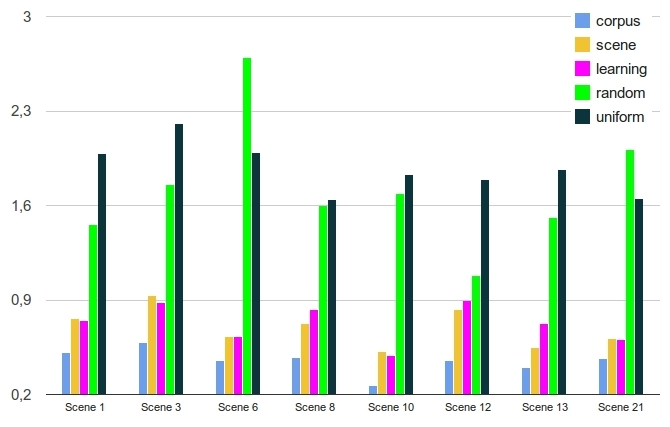
\includegraphics[width=.55\textwidth]{images/entropy.jpg}
\end{center}
\vspace*{-.5cm}
\caption{Cross-entropy between the corpus distribution and different runs of the algorithm}\label{Entropy}
\end{wrapfigure}

%Because accuracy is considered a very strict measure that in some cases can 
%be too stern on the evaluated algorithms 

%We also computed the entropy of the probability distribution of REs found in the corpus, and the cross-entropy between the corpus distribution of REs and the execution of each algorithm we just described~(see~\cite{juraksky:spee08} for details on cross-entropy evaluation). Figure~\ref{Entropy} shows the results for the eight scenes we are considering. 
%

Tambi\'en se calcul\'o la entrop\'{i}a de la distribuci\'on de probabilidad que se encuentro en el corpus, y la entrop\'{i}a cruzad entre la distribuci\'on del corpus de ER y las ejecuciones del algoritmo con las probabilidades que acabamos de describir~(ver~\cite{juraksky:spee08} para obtener detalles sobre evaluaci\'on de entrop\'{i}a cruzada). En la Figura~\ref{Entropy} se muestran los resultados para las ocho escenas que hemos considerado.

%
%The cross-entropies from the first two runs (\emph{scene} and \emph{learned}) are, in general, much closer to the corpus entropy than \emph{random}'s and \emph{uniform}'s cross-entropies, and to each other.  Only in Scene 12 \emph{random} approaches, by chance, the other two. 
%

Las entrop\'{i}as cruzadasde las dos primeras ejecusiones (\emph{escena} y \emph{aprendizaje autom\'atico}) son, en general, mucho m\'as cercanas de la entrop\'{i}a del corpus que las entrop\'ias cruzadas de \emph{random} y \emph{uniforme}. S\'olo la escena 12 \emph{enfoques aleatorios}, por casualidad, los otros dos.

%The figure clearly shows also that the cross entropies of \emph{scene} and \emph{learned} are in most cases very close to each other. 
%This observation supports the learning mechanism proposed in Section~\ref{sec:learning} to estimate the \puse\ when no corpora of REs of the target scene is available. 

\section{Evaluation} \label{sec:evaluation}

%In this section we present two different evaluations we performed on our algorithm. Section~\ref{sec:automaticevaluation} describes an evaluation with respect to the state of the art algorithm GRAPH~\cite{KrahmerGRAPH}. GRAPH was the top performer in both editions of the ASGRE, shared task~\cite{gatt-balz-kow:2008:ENLG}. Due to the limitations of the automatic metrics, in Section~\ref{sec:humanevaluation} we perform a human evaluation in  which we ask human subjects to compare the output produced by our algorithm to expressions produced by humans. 
%  
En esta secci\'on presentamos dos evaluaciones diferentes que realizamos en nuestro algoritmo. Secci\'on~\ref{sec:automaticevaluation} describe una evaluaci\'on con respecto al estado del arte~\cite{KrahmerGRAPH}. GRAPH fue el de mejor desempe\~no en las dos ediciones de la competencia ASGRE~\cite{gatt-balz-kow:2008:ENLG}. Debido a las limitaciones de los indicadores autom\'aticos, en la Secci\'on~\ref{sec:humanevaluation} realizamos una evaluaci\'on humana en la que pedimos sujetos humanos para comparar la salida producida por nuestro algoritmo de expresiones producidas por los seres humanos.
\subsection{Automatic evaluation} \label{sec:automaticevaluation}

%In this section we present the comparison of our algorithm to the state of the art algorithm GRAPH introduced above. The GRAPH algorithm is a deterministic algorithm and hence produces the same referring expression when run with the same target and model. Our algorithm is non deterministic, it may give a different referring expression each time it is run. In order to compare them we run our algorithm k times and we make a ranking of the top 20 produced referring expressions ordered by the frequency they were produced. We use the test part of the TUNA corpus to compare algorithm to the GRAPH algorithm whose results on this dataset are described in~\cite{KrahmerGRAPH} and reproduced in the Table~\ref{Tabla_sis_1_20}. 

%The GRAPH algorithm defines the generation of referring expressions as a graph search problem, which outputs the cheapest distinguishing graph (if one exists) given a particular cost function. We compare to this algorithm using the metrics accuracy, Dice and \textsc{masi}. Accuracy is defined as the percentage of exact matches between each ER produced by a human and the ER produced by the system for the same scene. 

%Dice coefficient is a set comparison metric, ranging between 0 and 1, where
%1 indicates a perfect match between sets. For two
%attribute sets A and B, Dice is computed as follows:\\

En esta secci\'on se presenta la comparaci\'on de nuestro algoritmo para el estado del arte GR\'AFICO algoritmo introducido anteriormente. El algoritmo GRAPH es un algoritmo determinista y por lo tanto produce la misma expresi\'on se refiere cuando se ejecuta con el mismo objetivo y modelo. Nuestro algoritmo es no determinista, puede dar una expresi\'on referencial diferente cada vez que se ejecuta. Con el fin de compararlos corremos nuestro tiempo k algoritmo y hacemos un ranking de los 20 mejores produjo refiri\'endose expresiones ordenados por la frecuencia que se produjeron. Utilizamos la parte de prueba del corpus AT\'UN comparar algoritmo para el algoritmo GR\'AFICO cuyos resultados en esta base de datos se describen en~\cite{KrahmerGRAPH} y reproducido en la tabla~\ref{Tabla_sis_1_20}.

El algoritmo GRAPH define la generaci\'on de expresiones que se refieren como un problema de b\'usqueda gr\'afica, que emite el gr\'afico distintivo m\'as barata (si existe) dada una funci\'on de coste particular. Comparamos a este algoritmo usando la precisi\'on m\'etrica, Dados y \textsc {masi}. La exactitud se define como el porcentaje de coincidencias exactas entre cada ER producido por un ser humano y el ER producido por el sistema para la misma escena.

Coeficiente de Dice es una m\'etrica comparaci\'on set, que oscila entre 0 y 1, donde
1 indica una combinaci\'on perfecta entre series. Para dos
atributo de los conjuntos A y B, dados se calcula como sigue:


$Dice(A,B) = \frac{2\times|A \cap B|}{|A|+|B|}$\\


The \textsc{masi} score \cite{Passonneau06measuringagreement}~is an adaptation of the Jaccard coefficient
which biases it in favor of similarity where one set
is a subset of the other. Like Dice, it ranges between
0 and 1, where 1 indicates a perfect match. It is computed as follows:\\


$\textsc{masi}(A,B) = \delta \times \frac{|A \cap B|}{|A \cup B|}$ \\


where $\delta$ is a monotonicity coefficient defined as follows:


 \begin{equation}
     \delta  = \left\{
	       \begin{array}{ll}
		 0      & if A \cap B = \emptyset \\
		 1 & if A = B  \\
		 \frac{2}{3}     & if A \subset B~or~B \subset A\\
		 \frac{1}{3}     & otherwise
	       \end{array}
	     \right.
 \end{equation}


Intuitively, this
means that those system-produced descriptions are
preferred which do not include attributes that are
omitted by a human.  

In Table~\ref{Tabla_sis_1_20} we show the automatic metrics and compare the performance of our system  with the GRAPH system for the first ER in the ranking and the first 20 REs in the ranking. 

\begin{table}[h!]
\begin{center}
\begin{tabular}{|l|c|c|c|}
\hline
%Figure & Model \puse &  Learning \puse & Random \puse &  Uniform \puse \\
	 	& 	Dice		&	\textsc{masi}	&	ACCURACY		\\
\hline
GRAPH system, Furniture domain	& 	.80 		&	.59	&	.48		 	\\
GRAPH system, People domain 	& 	.72		&	.48	&	.28			\\
\hline
Our system, Furniture domain (top 1)	&	.80		&	.60	&	.47		\\
Our system, People domain (top 1)	&	.65		&	.37	&	.19		\\
\hline
Our system, Furniture domain (top 20)&	.87		&	.75  	&	.65		\\
Our system, People domain (top 20)   &	.81		&	.68	&	.60		\\
\hline
\end{tabular}
%\vspace*{.1cm}
\caption{Comparison of the GRAPH algorithm and our system. We consider the 3 automatic metrics for the top 1 and the top 20 REs produced by our algorithm.}
\vspace*{-.5cm}
\label{Tabla_sis_1_20}
\end{center}
\end{table}
\vspace*{-.5cm}
%Accuracy, Dice and \textsc{masi} assess humanlikeness with respect to a corpus of human referring expressions. In the Figure~\ref{graficoPresicion} the accuracy for our system and the GRAPH system is compared. The left GRAPH corresponds to the furniture domain and the right GRAPH corresponds to the people domain. We can see that taking the top 1 ER our system accuracy is lower than GRAPH performance for the people domain. However, if we consider the top 20 REs that our algorithm is able to produce we can see that the accuracy for both domains gets higher than 60\%. This shows that our algorithm is able to generate REs that are more similar to those produced by humans than the GRAPH algorithm, although these REs are not ranked first. 

%Another result that we can observe is that the people domain accuracy is much lower for the top 1 ER than for the furniture domain (19 vs 47), but the accuracy stabilizes when REs lower in our ranking are considered. This may be explained by the fact that the training set for the people domain is smaller and less balanced and hence, the probabilities of use inferred do not generalize as well as in the furniture domain. 


Precisi\'on, Dados y \textsc{masi}  evaluar humanlikeness con respecto a un corpus de expresiones humanas en referencia. En la figura~\ref{graficoPresicion} la precisi\'on de nuestro sistema y el sistema GRAPH se compara. El gr\'afico de la izquierda corresponde al dominio muebles y el gr\'afico de la derecha corresponde al dominio personas. Podemos ver que la toma de la parte superior 1 ER nuestra precisi\'on del sistema es menor que el rendimiento gr\'afico para el dominio de las personas. Sin embargo, si tenemos en cuenta los 20 mejores ER que nuestro algoritmo es capaz de producir, podemos ver que la precisi\'on de ambos dominios se hace mayor del 60 \%. Esto demuestra que nuestro algoritmo es capaz de generar REs que son m\'as similares a los producidos por los seres humanos que el algoritmo GRAPH, aunque estos REs no se clasifican primero.

Otro resultado que podemos observar es que la exactitud de dominio personas es mucho menor para el 1 ER que para el dominio de muebles (19 vs 47), pero la precisi\'on estabiliza cuando se consideran ER inferiores en nuestro ranking. Esto puede explicarse por el hecho de que el conjunto de entrenamiento para el dominio de la gente es m\'as peque\~no y menos equilibrado y por lo tanto, las probabilidades de uso inferido no generalizar, as\'{i} como en el dominio de muebles.

\begin{figure}[ht]
\begin{minipage}{0.50\linewidth}
\centering
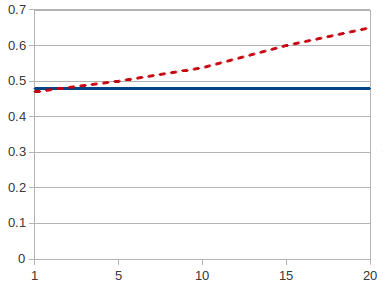
\includegraphics[width=\textwidth]{images/furniturePrec.png}
%\end{figure}
\end{minipage}
%\begin{figure}[ht]
\begin{minipage}{0.50\linewidth}
\centering
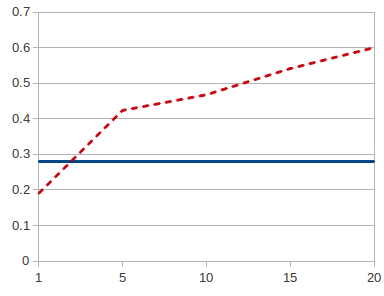
\includegraphics[width=\textwidth]{images/precP.png}
\end{minipage}
\caption{Comparison of the accuracy of the GRAPH algorithm and our system. The x axis indicates that the accuracy was calculated considering the x first REs in the ranking. The y axis indicates the accuracy. Our system is depicted as a dotted line and the GRAPH system as a continuous line.\label{graficoPresicion}}
\end{figure}

 
%\vspace*{-1.0cm}

\subsection{Human evaluation} \label{sec:humanevaluation}

%We asked two native speaker judges of English to evaluate our referring expressions via an experiment on the web. The authors of the paper did not participate during the evaluation. The judges could register to the evaluation system so that they did not have to complete it in one go, the could come back to it later. During the evaluation we showed each judge the scenes and two randomly ordered REs. One ER corresponded to the ER present in the corpus and produced by a person and the other ER corresponded to the top 1 ER produced by our system. We asked the judges to select the ER that would be more useful to identify the target in the scene. That is, to select it from among the other objects in the stimulus pictures. 

%Our goal is to show that even if the ER generated by our algorithm does not coincide with the ER produced by a human in the corpus collection, it can be judged as good or even better than the REs generated by humans. 

%In Table~\ref{system-versus-human} we show the results from the human evaluation experiment.
%The REs produced by the system were considered equal or better by both
%judges in 60 \% of the cases and, by at least one judge in 92\% of the cases.

Pedimos dos jueces nativos de Ingl\'es para evaluar nuestras expresiones referidas a trav\'es de un experimento en la web. Los autores del trabajo no participaron en la evaluaci\'on. Los jueces podr\'{i}an registrarse en el sistema de evaluaci\'on a fin de que no ten\'{i}an que terminarlo de una vez, la podr\'{i}a volver a ella m\'as tarde. Durante la evaluaci\'on demostramos cada juez de las escenas y dos ER ordenadas al azar. Uno ER correspondi\'o a la ER presente en el corpus y producido por una persona y la otra ER correspondi\'o al 1 ER superior producida por nuestro sistema. Preguntamos a los jueces para seleccionar el ER que ser\'{i}a m\'as \'util para identificar el blanco en la escena. Es decir, para seleccionarlo de entre los otros objetos en las fotos de est\'{i}mulo.

Nuestro objetivo es mostrar que incluso si el ER generada por nuestro algoritmo no coincide con la ER producido por un ser humano en la colecci\'on corpus, puede ser juzgado como bueno o incluso mejor que las REs generados por los seres humanos.

En la tabla~\ref{sistema-contra-humana} se muestran los resultados del experimento de evaluaci\'on humana.
Las ER producidos por el sistema se consideraron igual o mejor por tanto
jueces en 60 \% de los casos y, por lo menos un juez en 92 \% de los casos.

\begin{table}[h!]
\begin{center}
\begin{tabular}{|l|c|c|c|c|}
\hline
%total scenes in evaluation set &                           80   &             68
 & Furniture domain & People domain & Weighted mean \\
\hline
system equal to human  	&	.46	&	.19	&	.33 \\
system better by 2 judges &	.29 	& 	.24 	& 	.27 \\
system better by 1 or 2 judges & .51	&	.68	&	.59 \\
system worse by 2 judges &	.03	&	.13	&	.08 \\
system equal or better by 2 judges  &.75  &       .43	&       .60 \\
system equal or better by 1 judge  &.97	&	.87	&	.92 \\
\hline
\end{tabular}
%\vspace*{.1cm}
\caption{Percentage of system versus human selected choices} 
\label{system-versus-human}
\vspace*{-.5cm}
\end{center}
\end{table}

%Below, we illustrate the evaluation experiment by showing examples of cases in which the system expression was considered better by both judges, by only one judge or by neither of them. 

%Figure~\ref{smallBlueFan} illustrates a case in which the human generated an underspecified ER while the system produced an ER which unequivocally identifies the target. The ER generated by the system for this figure is ``small blue fan'' while the ER produced by the human is ``blue fan''. The human ER fails to uniquely identify the target and is then not preferred by the human judges. Humans are known for producing underspecified REs which may be due to cognitive limitations for not being able to consider the whole referential context at the same time. Our algorithm is able to consider the whole referential context and combine this ability with the probability of use of the REs learned from humans. 

A continuaci\'on, se ilustra el experimento de evaluaci\'on, mostrando ejemplos de casos en los que la expresi\'on sistema fue considerado mejor por ambos jueces, por un solo juez o por ninguno de los dos.

Figura~\ref{smallBlueFan} ilustra un caso en el que el humano genera un ER underspecified mientras el sistema produce un ER que identifica de manera inequ\'{i}voca el objetivo. El ER generada por el sistema para esta figura es `` peque\~no ventilador azul '', mientras que el ER producido por el ser humano es `` ventilador azul ''. El ER humano no logra identificar de forma \'unica el objetivo y es entonces no preferido por los jueces humanos. Los seres humanos son conocidos por producir ER underspecified que puede ser debido a las limitaciones cognitivas por no ser capaz de considerar todo el contexto referencial, al mismo tiempo. Nuestro algoritmo es capaz de considerar todo el contexto referencial y combinar esta capacidad con la probabilidad de uso de las ER aprendido de los seres 

\begin{figure}[h]
\begin{minipage}{0.48\linewidth}
\centering
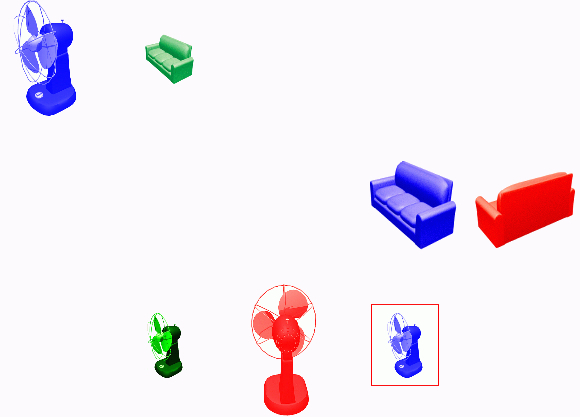
\includegraphics[width=\textwidth]{images/smallBlueFan.jpg}
\caption{Scene used during the collection of the TUNA corpus. The human ER \emph{blue fan}, and the system \emph{small blue fan}. Judges prefer the system generated.}
\label{smallBlueFan}
\end{minipage}
\hspace*{.04cm}
\begin{minipage}{0.48\linewidth}
\centering
\vspace*{.4cm}
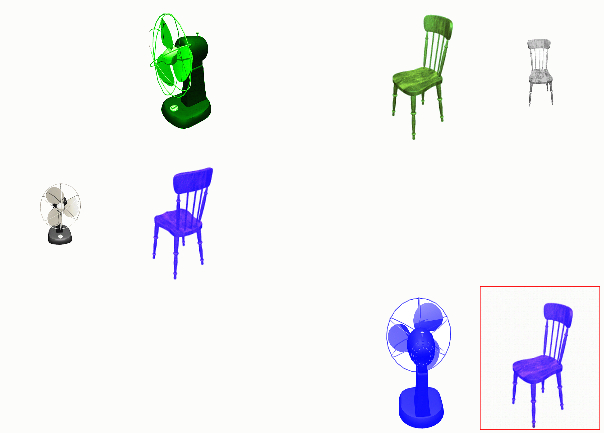
\includegraphics[width=\textwidth]{images/tuna.jpg} % esta es la 101t5 la que mostramos al principio
\vspace*{-.4cm}
\caption{Scene used during the collection of the TUNA corpus. The human ER was \emph{blue frontal chair}, and the system \emph{the blue chair in the bottom}. Both human judges prefer the system generated RE.}
\label{BlueChair}
\end{minipage}
\end{figure}


%In Figure~\ref{BlueChair} the human ER was ``blue frontal chair'', and the system ER was ``the blue chair in the bottom''; both judges selected the system RE. This case can be explained by the fact that, in this domain, the property ``bottom'' helps more during the identification than the property ``frontal'' because it concentrates the attention of the interpreter in the lower part of the scene. Our system learns this fact by learning a higher value of \puse~for ``bottom'' than for ``frontal'' from the training data. 

En la figura~\ref{BlueChair}  el ER humana era `` silla frontal azul '', y el ER sistema era `` la silla azul en la parte inferior ''; ambos jueces seleccionaron el ER sistema. Este caso se puede explicar por el hecho de que, en este \'ambito, la propiedad '' inferior '' ayuda a m\'as durante la identificaci\'on de la propiedad '' frontal '' porque concentra la atenci\'on del int\'erprete en la parte inferior de la escena. Nuestro sistema aprende este hecho por el aprendizaje de un mayor valor de \ puse~por `` abajo '' que para `` frontal '' a partir de los datos de entrenamiento.

\begin{figure}[h]
\begin{minipage}{0.48\linewidth}
\centering
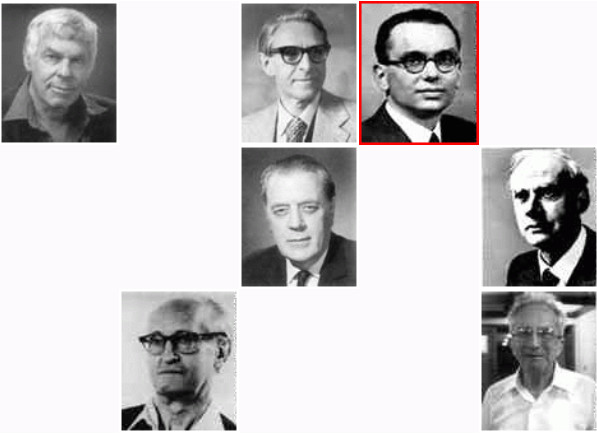
\includegraphics[width=\textwidth]{images/s59t26.jpg}
\caption{Scene used during the collection of the TUNA corpus. The human  ER was \emph{the man with black hair}, and the system \emph{the man wearing glasses in the fourth column}. Judges prefer the human RE.}
\label{s28t25}
\end{minipage}
\hspace*{.04cm}
\begin{minipage}{0.48\linewidth}
\centering
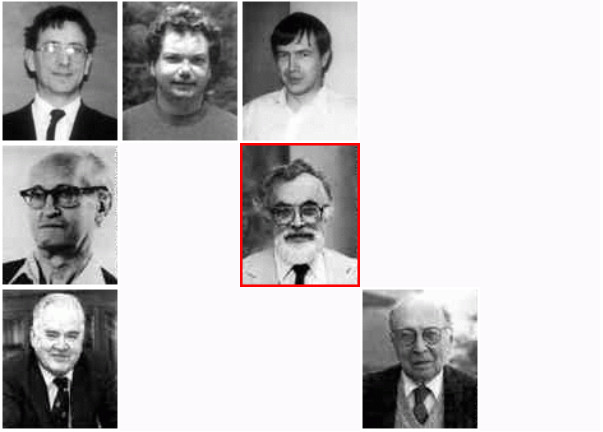
\includegraphics[width=\textwidth]{images/s315t21.jpg}
\vspace*{-.3cm}
\caption{Scene used during the collection of the TUNA corpus. The human ER was \emph{man with a beard}, and the system \emph{man with a beard wearing glasses}. Judges did not agree in their preference.}
\label{s307t21}
\end{minipage}
\end{figure}

%Figure~\ref{s28t25} is an example for which both judges preferred the human expression. The human  ER was ``the man with black hair'', and the system's ``the man wearing glasses in the fourth column''. This example makes evident the fact that, in the people domain some properties are more salient in some images than in others because of different shades of colors. Gradable properties such as this ones (in contrast to absolute properties) are still an open problem for GRE algorithms. 

%Figure~\ref{s307t21}~illustrates a case in which the system ER was more overspecified than the human RE; the system included ``wearing glasses'' while the human did not. In this case one human subject preferred the system ER and the other the human RE. The amount of overspecification is a subjective matter where human themselves disagree. Further evaluation where REs are actually used for a task would be interesting to investigate this issue.  


Figura~\ref{s28t25} es un ejemplo para los que ambos jueces prefieren la expresi\'on humana. El ER humana era `` el hombre con el pelo negro '', y del sistema de `` el hombre con gafas en la cuarta columna ''. Este ejemplo pone de manifiesto el hecho de que, en el dominio de la gente algunas propiedades son m\'as destacada en algunas im\'agenes que en otros debido a diferentes tonos de colores. Propiedades graduables como este queridos (en contraste con las propiedades absolutas) son todav\'{i}a un problema abierto para los algoritmos GRE.

Figura~\ref{s307t21}~ilustra un caso en el que el ER sistema era m\'as falte espacio que el ER humana; el sistema incluye `` con gafas '', mientras que el ser humano no lo hizo. En este caso un sujeto humano prefiere el sistema de ER y el otro el ER humano. La cantidad de especificaci\'on excesiva es una cuesti\'on subjetiva, donde humana mismos no est\'an de acuerdo. Una evaluaci\'on m\'as profunda donde ER se utilizan realmente para una tarea ser\'{i}a interesante investigar este asunto.

